%----------------------------------------------------------------------------------------
%	PACKAGES AND OTHER DOCUMENT CONFIGURATIONS
%----------------------------------------------------------------------------------------
\documentclass[a4paper,11pt]{article}

%Include Packages
%----------------------------------------------------
\usepackage{../Header/KaTeX_LabReport}
\usepackage{lipsum}
% Note: 
% The input command is equivalent to copy-paste the content of the file
% into the current file.

\renewcommand{\thesection}{\Roman{section}} 
\titleformat{\section}[display]%command shape
    {\Huge}%format
    {
        \newpage
        \setlength\fboxsep{0pt}
        \color{gray} \fontsize{20}{5}\selectfont\chaptername\ \thesection
    }%label
    {0pt}{}{}
\titlespacing*{\section}{0pt}{0pt}{20pt}
\renewcommand{\thesubsection}{\thesection: \Roman{subsection}}
\renewcommand{\thesubsubsection}{\thesubsection. \roman{subsubsection}}
\renewcommand{\thesubsection}{\Roman{subsection}}
\titleformat{\subsection}
    {\bfseries\Large}%format
    {\huge\textnormal{\thesubsection}}%label
    {12pt}{}{}

\usepackage{sectsty}
    \sectionfont{\LARGE}
    \subsectionfont{\large}
    \subsubsectionfont{\large}
    \paragraphfont{\large}
\usepackage{titletoc}
    \titlecontents{}[1em]{\addvspace{1pc}\bfseries}      {\contentslabel{3em}}{}
    {\titlerule*[0.3pc]{.}\contentspage}

\usepackage{tocloft}% http://ctan.org/pkg/tocloft
\setlength\cftsecnumwidth{6em}

\renewcommand{\thesubsubsection}{\thesubsection: \roman{subsubsection}}
\titlespacing{\subsubsection}{0pt}{15pt}{5pt}

%Hyperlink Setting
%----------------------------------------------------
\hypersetup{hidelinks,
	colorlinks=true,
	allcolors=black,
	pdfstartview=Fit,
	breaklinks=true
}

% \includeonly{
%     Experiment_01/Lab1_Main,
%     Experiment_02/Lab2_Main,
%     Experiment_07/Lab7_Main,
% }

\begin{document}
%----------------------------------------------------------------------------------------
%	FRONT MATTER
%----------------------------------------------------------------------------------------
% Cover
\thispagestyle{empty}
\begin{titlepage}
    % Warning Filter
    \WarningFilter[latex]{latexfont}{Some font shapes}
    \WarningFilter[latex]{tex}{Underfull \hbox}
    \ActivateWarningFilters[latex]

	%\hspace{0.05\textheight} % Whitespace between the vertical line and title page text
    \parbox{1\textwidth}{ % Paragraph box for holding the title page text, adjust the width to move the title page left or right on the page
		{\Huge\bfseries EIE420 Assignment II \\[0.15\baselineskip] 
        Gray Scale Histrogram}\\[0.15\baselineskip] % Title
		\rule{1\textwidth}{1pt} % Vertical line
        {\Large\textit{Report of EIE420, Digital Image Processing Assignment}}
        \newline
    }
    \parbox{1\textwidth}{
        \vspace{1\baselineskip}
        \large
        Source Code of this assignment could be found at:\newline
        \url{https://github.com/ZeppelinSCB/EIE420-Digital_Image_Processing}
        \newline
    }
    \vspace{100pt} % Whitespace between the title block and the publisher
    \parbox{1\textwidth}{
        {\large by}\\[1.5\baselineskip]
        {\rule[1pt]{200pt}{1pt}} \\[1.25pt]
        {\huge\textsc{Pengrui K. Tong}
            %\begin{CJK*}{UTF8}{bsmi}\Large (湯鵬睿)\end{CJK*}
            }\\
        {\large{Student No: 1220031811}} \\
        \large from EIE420 D1, \newline
        Faculty of Innovation Engeneering, \newline
        Universidade de Ciência e Tecnologia de Macau
    }
		

    \vspace*{\fill}
		Apr 6, 2025 \newline 
        (Coloane, Macao, SAR)
        \vspace{0.7\baselineskip}\newline
        %
\includegraphics[width = 40mm]{MUIT_BlueGold.png}\newline
        
\includegraphics[width = 40mm]{../Header/MUIT_origin.png}\par
        {\small Cover Design by Karl Tong}\\[0.25pt]
        {\small This report is a part of the result for}
        {\small EIE420~Digital~Image~Processing in U.C.T.M}\\[0.25pt]
        {\small \copyright 2025 Pengrui Tong}
\end{titlepage}
\blankpage

% Table of Contents
\tableofcontents
\blankpage

\section{Problem Statement}
Two fairly simple task was assigned to help understand basic operation of image in Matlab. \\
\subsection{Objective}
    In this experiment, we want to implement two funcions. One is to split and display different channel of a multi-channel image, this is usefull when we want to inspect an image channel by channel. The other is to cutout a sub-image from a given image, this is useful when we want to focus on a specific part of the image.\\

\section{Procedure}
Apparantly, this task requires me to implement two funcions. So I wrote two matlab function, and a main script to processe an image with those functions.

\subsection{Design of the Channel split function}
\subsubsection{Function description}
Besides fullfill the basic requirements, my funciton also capable to dealwith image with any number of channel.
\begin{enumerate}
    \item Check and save the size of the input image.
    \item Create the output matrix and filled with 0, with the size vairous with the size of channel to fit all of them. This means this funciton can deal with image with any number of channel.
    \item Traversal all channels, and copy only the channel we want to display to the new matrix.
    \item Return the result matrix
\end{enumerate}
\subsubsection{Designed IO}
\subsubsection*{Input}
\textbf{image}: \\
Image input. An uint8 format matrix with three dimention.
\subsubsection*{Output}
\textbf{imOut}: \\
Output image. An uint8 format matrix with three dimention, and contains the original image as well as the splited channel in the order of the channel's index.

\subsection{Design of the Image Cut function}
\subsubsection{Function description}
Besides fullfill the basic requirements, I achive polymorphism by threating input as an array, and different the response for different number of input paramter.
\begin{enumerate}
    \item Detect the number of input to switch area selecting steyle between "point-size" or "point-point". 
    \item "Point-size" mode would be excecuted if five input was detected. In this mode, the function will return the area started at the given point, and with the given size.
    \item "Point-Point" mode would be excecuted if three input was detected. In this mode, the funciton will return the subfigure between two point.
    \item If the number of input paramters isn't valid, an error will be thrown.
\end{enumerate}
\subsubsection{Designed IO}
\subsubsection*{Input}
\textbf{image, startR, startC, sizeR, sizeC}\\
The input image; the row and colum coordinate of the starting point; the size in row and colum respectively. Note all the unit is pixel.
\textbf{image, startR, startC, endR, endC}\\
The input image; the row and column coordinate of the starting point; and the coordinate of the ending point. Note all the units are in pixels.
\subsubsection*{Output}
\textbf{imOut}:\\
Output image. An uint8 format matrix that contains the sub-image extracted from the input image based on the specified coordinates or size.

\section{Source Code}
\subsection{Main Program Code}
\lstset{language = Matlab}
    \begin{lstlisting}[basicstyle=\tiny]
        clc;
        IMAGE = "Anon.jpg";
        FOLDER = "work/";
        PATH = append(FOLDER,IMAGE);
        Start = [193, 709];
        
        iSource = imread(PATH);
        [r,c,k] = size(iSource);
        subplot(1,3,1);
        imshow(iSource);
        title('Original Image');
        axis on;
        
        imgSplit = GetColorCom(iSource);
        subplot(1,3,2)
        imshow(imgSplit)
        title('Channel Split Image');
        axis on;
        
        imgCut = GetSubImage(iSource,[200 700],[600 1100]);
        subplot(1,3,3);
        imshow(imgCut);
        title('Image Segment');
        axis on;
        
        impixelinfo;
\end{lstlisting}

\subsection{Code for Split Channel}
\lstset{language = Matlab}
    \begin{lstlisting}[basicstyle=\tiny]
        function imOut = GetColorCom(image)
        [y,x,k]=size(image);
        imOut = zeros((floorDiv(k,2)+1),2*x,k,"uint8");
        imOut(1:y,1:x,:)=image(:,:,:);
        for i=1:k
            row = floorDiv(i,2);%number of rows, start from 0
            col = mod(i,2);%0 for even, 1 for odd
            imOut((1+row*y):((row+1)*y),(1+col*x):((col+1)*x),i)=image(:,:,i);
        end
        end
\end{lstlisting}

\subsection{Code for Cutting image}
\lstset{language = Matlab}
    \begin{lstlisting}[basicstyle=\tiny]
        function imOut = GetSubImage(varargin)
        disp(length(varargin));
        if(length(varargin)==5)
            imgIn=varargin{1};
            startR=varargin{2};
            startC=varargin{3};
            sizeR=varargin{4};
            sizeC=varargin{5};
            imOut = imgIn(startR:(startR+sizeR),startC:(startC+sizeC),:);
        elseif(length(varargin)==3)
            imgIn=varargin{1};
            startR=varargin{2}(2);%Start(x,y)
            startC=varargin{2}(1);%Start(x,y)
            endR=varargin{3}(2);%Start(x,y)
            endC=varargin{3}(1);%Start(x,y)
            imOut = imgIn(startR:endR,startC:endC,:);
        else
            display("Invalid Number of Inputs")
        end
        end
\end{lstlisting}

\section{Discussion}
\subsection{Sample Program Output}
Running the main script, we get the following result. Please note I run the main script twice with difference parameter to demonstrade the cut image function actually works with different input paramters.
\begin{figure}[H]
    \centering
    \begin{subfigure}{0.8\textwidth}
        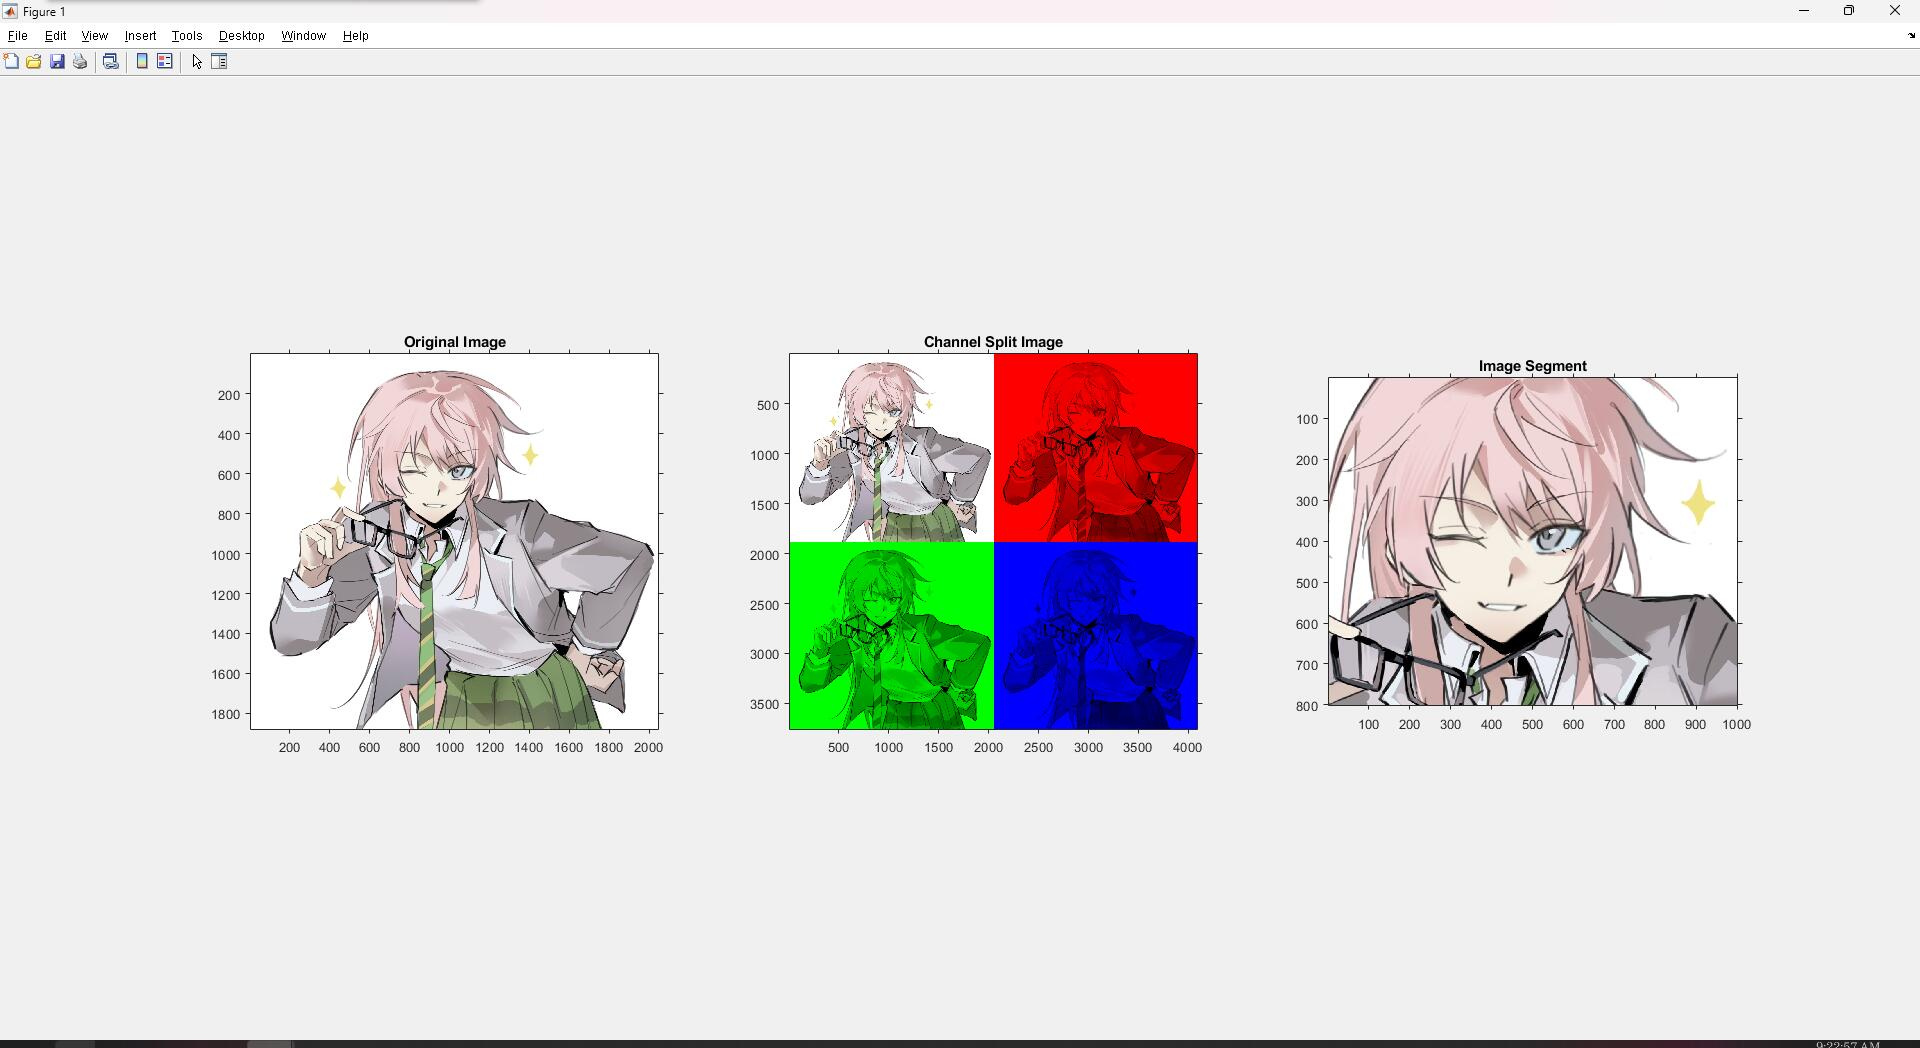
\includegraphics[width=1\linewidth]{Demo1-Head.jpg}
        \caption{Demo Image I}
        \label{pic:d1}
    \end{subfigure}

    \begin{subfigure}{0.8\textwidth}
        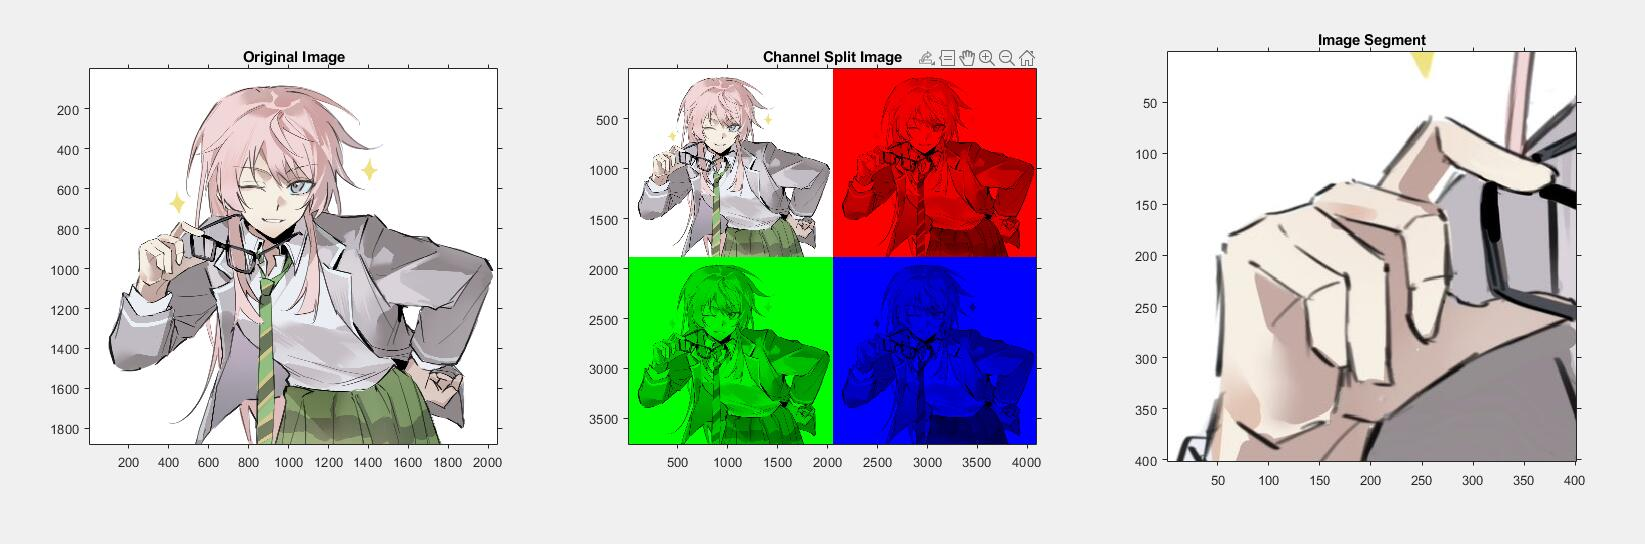
\includegraphics[width=1\linewidth]{Deme2-Hand.jpg}
        \caption{Demo Image II}
        \label{pic:d2}
    \end{subfigure}
    \caption{Two demonstration images}
\end{figure}
From the figure above, we can see the in both demo, the channel split functions works as intended. And we can see from fig \ref{pic:d1} and fig\ref{pic:d2} that the image cut funtion can caputre with different style of input parameter.

\section{Conclusion}
In conclusion, I successfully implemented two functions in Matlab to split image channels and cut out sub-images. Through this assignment, I learned how to manipulate multi-channel images and handle different input parameters to achieve polymorphism in function design. This exercise enhanced my understanding of basic image processing operations in Matlab.

\section{References}
No outside sources was referened expect the lecture notes and the matlab official doucumentation.
\end{document}